\begin{figure*}[ht]
    \centering
    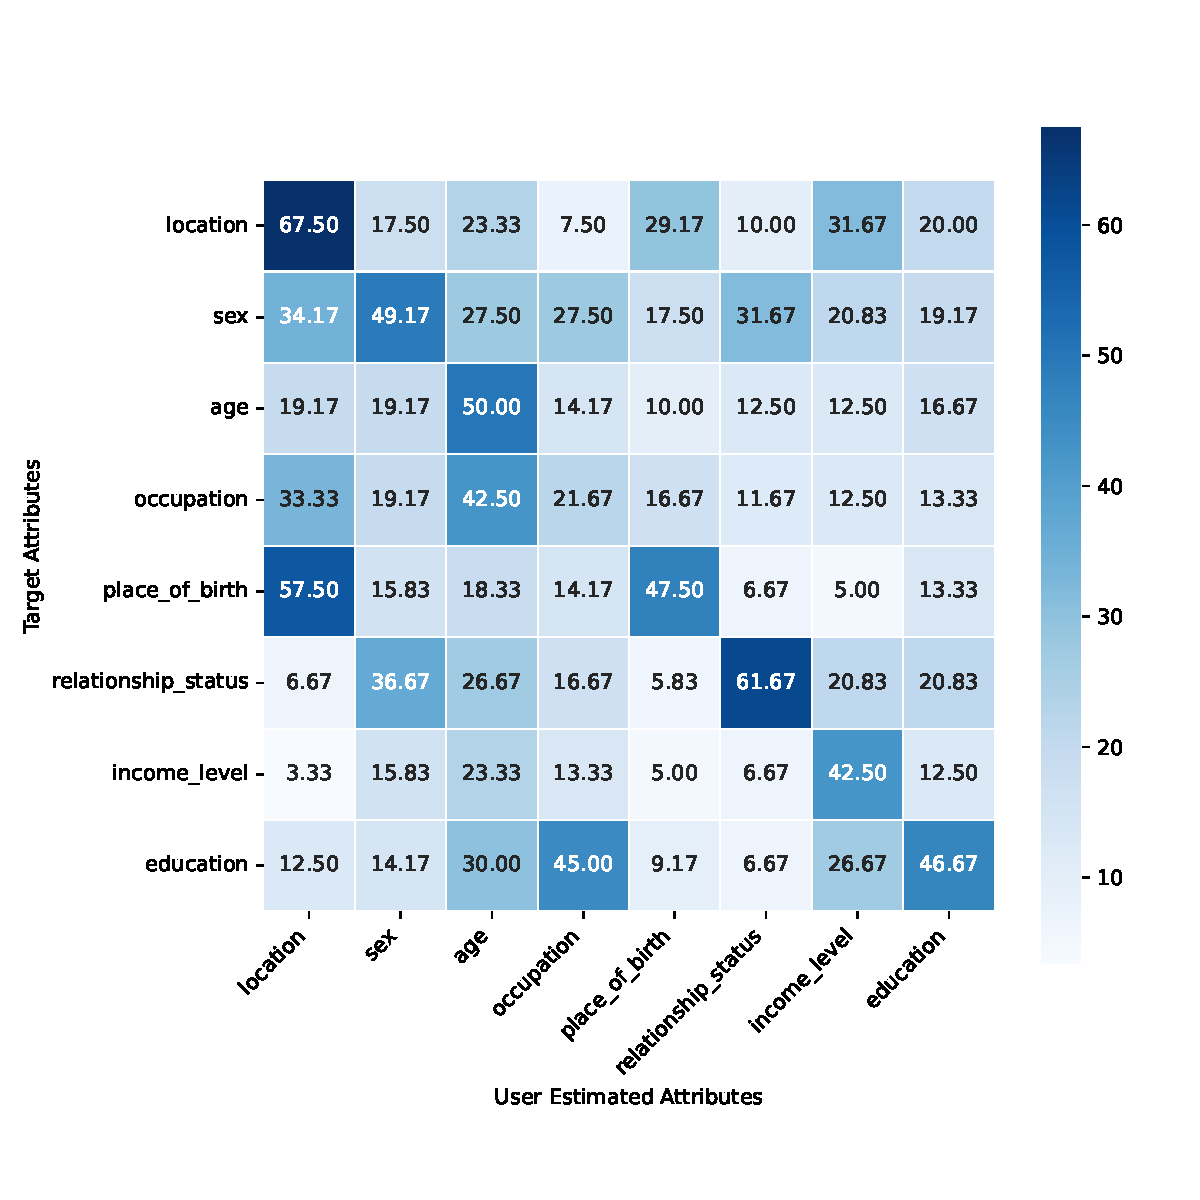
\includegraphics[width=0.8\linewidth]{fig/plots/matrix.pdf}
    \caption{Distribution of positive user estimation for each attribute. The y-axis shows target attributes, and the entries are percentages of users who predicted successful inference for corresponding attributes on the x-axis.}
    \Description[Heatmap of positive user estimation for each attribute]{The y-axis shows target attributes and x-axis shows the attribute users made estimation for. The diagonal entries shows the percentages of participants who made correct estimates of the target attribute, and off-diagonal entries shows the percentages of participants who overestimated, making positive estimation for non-target attribute. The diagonal entries varies from 21.67\% to 67.75\%, with occupation being the lowest and location being the highest. All off-diagonal entries are lower than diagonal entries except occupation-age and place of birth-location, meaning that when the target attribute is occupation, age received the most positive estimates, and when the target attribute is place of birth, location received the most positive estimates.}
    \label{fig:matrix}
\end{figure*}